\documentclass{article}
\usepackage[utf8]{inputenc}

\title{Coursework2019 - EEE6205}
\author{Group 5}
\date{November 2019}

\usepackage{natbib}
\usepackage{graphicx}
\usepackage{subcaption}
\usepackage{float}

\begin{document}

\maketitle

\section*{1a} 
For six step operation the fundamental component is given in Equation: \ref{equ:SSP}.
\begin{equation}
    \frac{V_{Ph-Ph}}{V_{Ph-N}}=\frac{2 \sqrt{3}}{\pi}
\label{equ:SSP}
\end{equation}
Using sinusoidal pulse width modulation (SPWM) instead them maximum fundamental component is given in Equation: \ref{equ:SPWM}. This is achieved on the border of over-modulation where the sinusoidal peak meets the PWM peak voltage, anything under-modulated would reduce the fundamental component. 
\begin{equation}
\frac{V_{Ph-Ph}}{V_{Ph-N}}=\frac{\sqrt{3}}{2}
    \label{equ:SPWM}
\end{equation}
To increase the fundamental component as much as possible six step operation should be used.


\section*{1b} 

The results of using six step mode can be see in in Figure:\ref{fig:fig1} with a fundamental peak at 1.1027 as expected by Equation:\ref{equ:SSP}.
\begin{figure}[H]
\begin{subfigure}{.5\textwidth}
  \centering
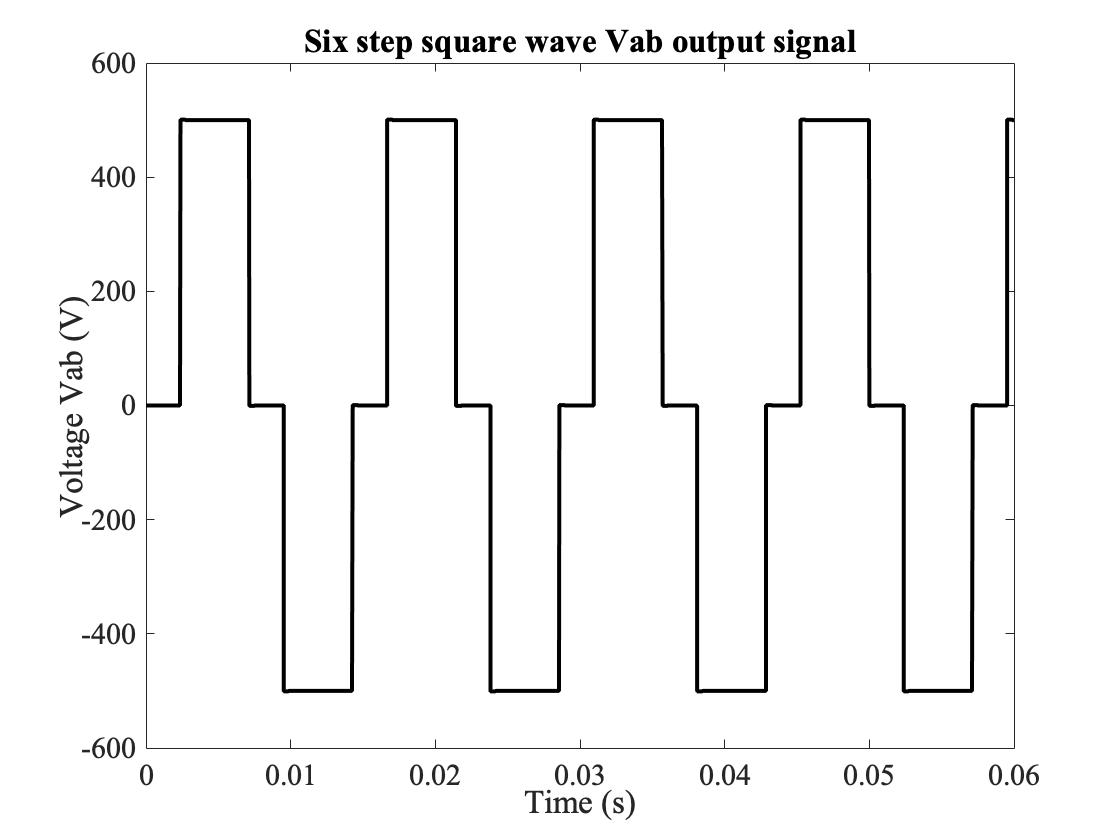
\includegraphics[scale=0.15]{one.jpg}
\caption{V_{ab} of six step inverter}
\label{fig:signalOne}
\end{subfigure}%
\begin{subfigure}{.5\textwidth}
  \centering
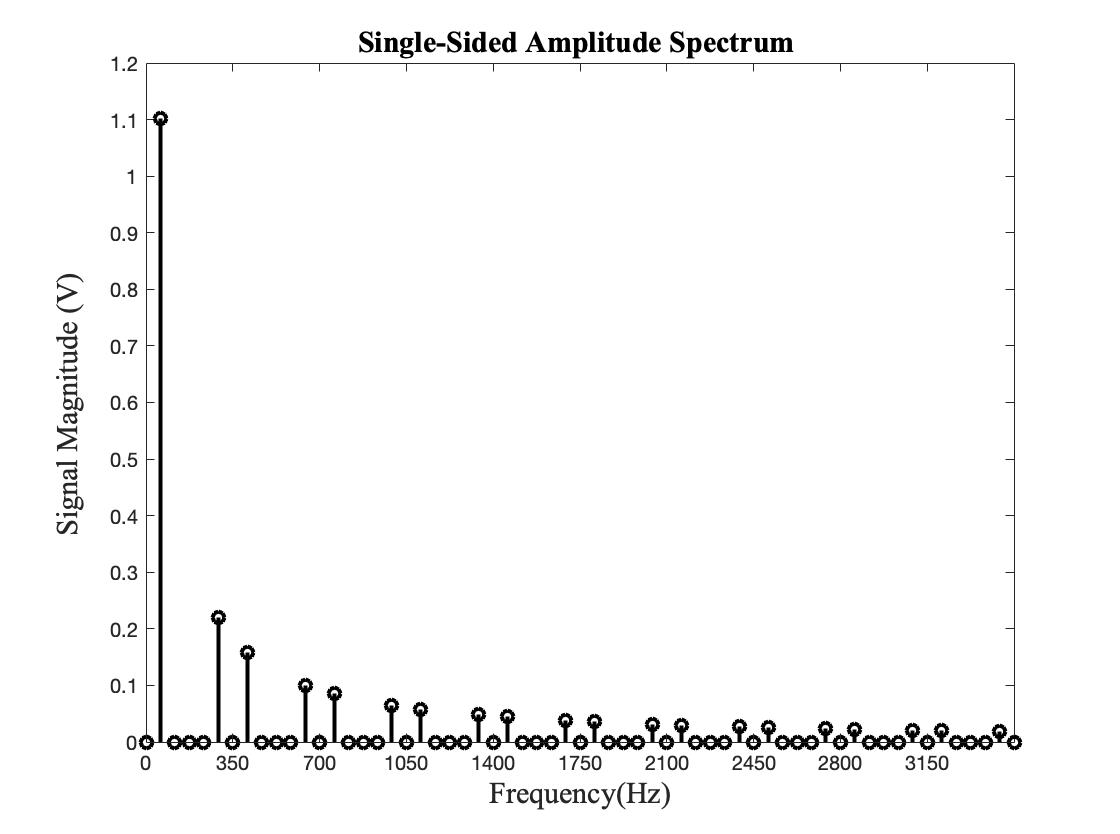
\includegraphics[scale=0.15]{two.jpg}
\caption{FFT of signal in Figure:\ref{fig:signalOne}}
\label{fig:fftOne}
\end{subfigure}
\caption{$V_{ab}$ Six step square wave signal and Fourier Transform}
\label{fig:fig1}
\end{figure}

The results of using SPWM can be see in in Figure:\ref{fig:fig2} with a fundamental peak at 0.8655 roughly equal to that of Equation:\ref{equ:SPWM}.
\begin{figure}[H]
\begin{subfigure}{.5\textwidth}
  \centering
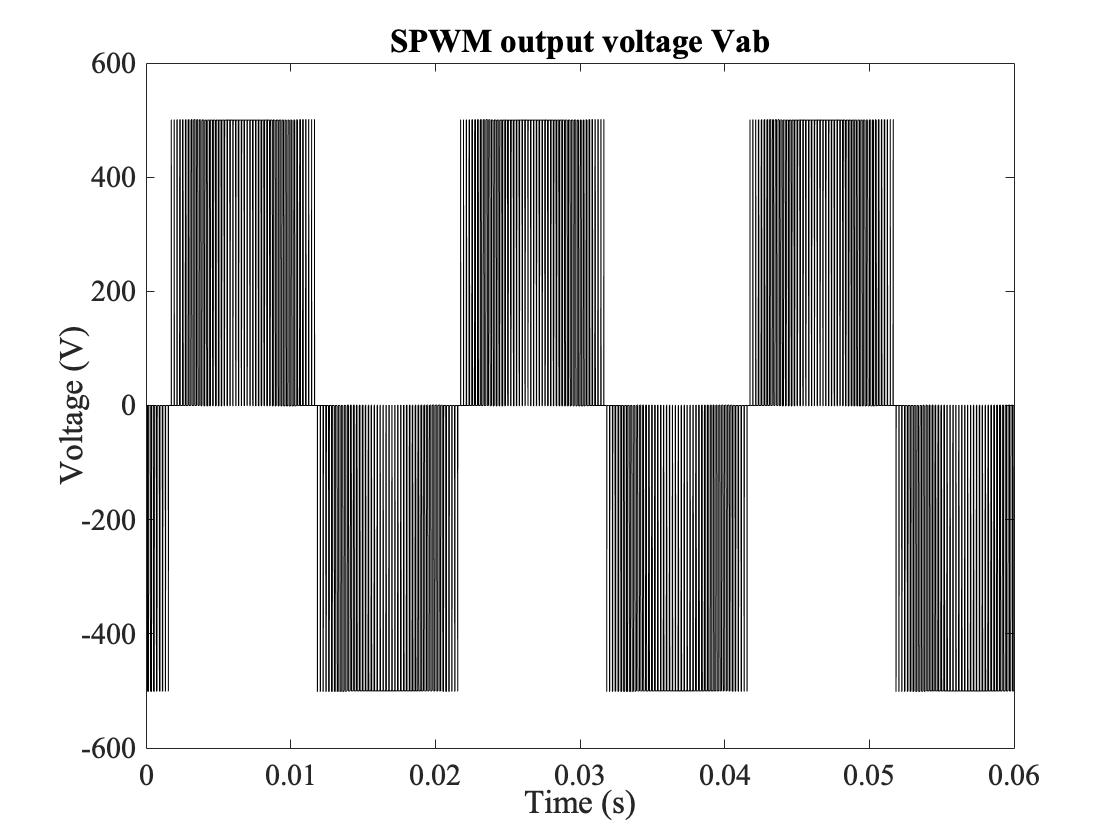
\includegraphics[scale=0.15]{three.jpg}
\caption{V_{ab} of SPWM inverter}
\label{fig:signalTwo}
\end{subfigure}%
\begin{subfigure}{.5\textwidth}
  \centering
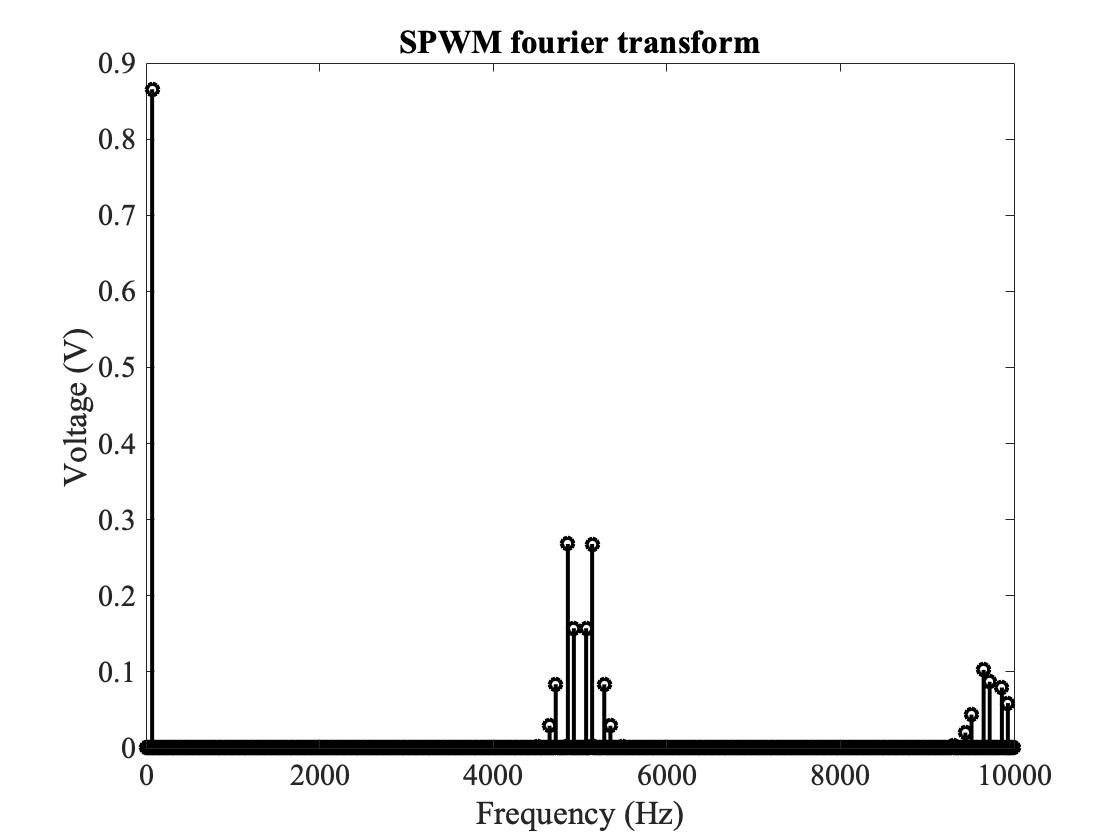
\includegraphics[scale=0.15]{four.jpg}
\caption{FFT of signal in Figure:\ref{fig:signalTwo} }
\label{fig:fftOne}
\end{subfigure}
\caption{$V_{ab}$ SPWM signal and Fourier Transform}
\label{fig:fig2}
\end{figure}

\section*{1c} 
All switches in the device, whilst operating in six step mode, operate at the signal frequency ($70Hz$). 
\begin{figure}[H]
\begin{subfigure}{.5\textwidth}
  \centering
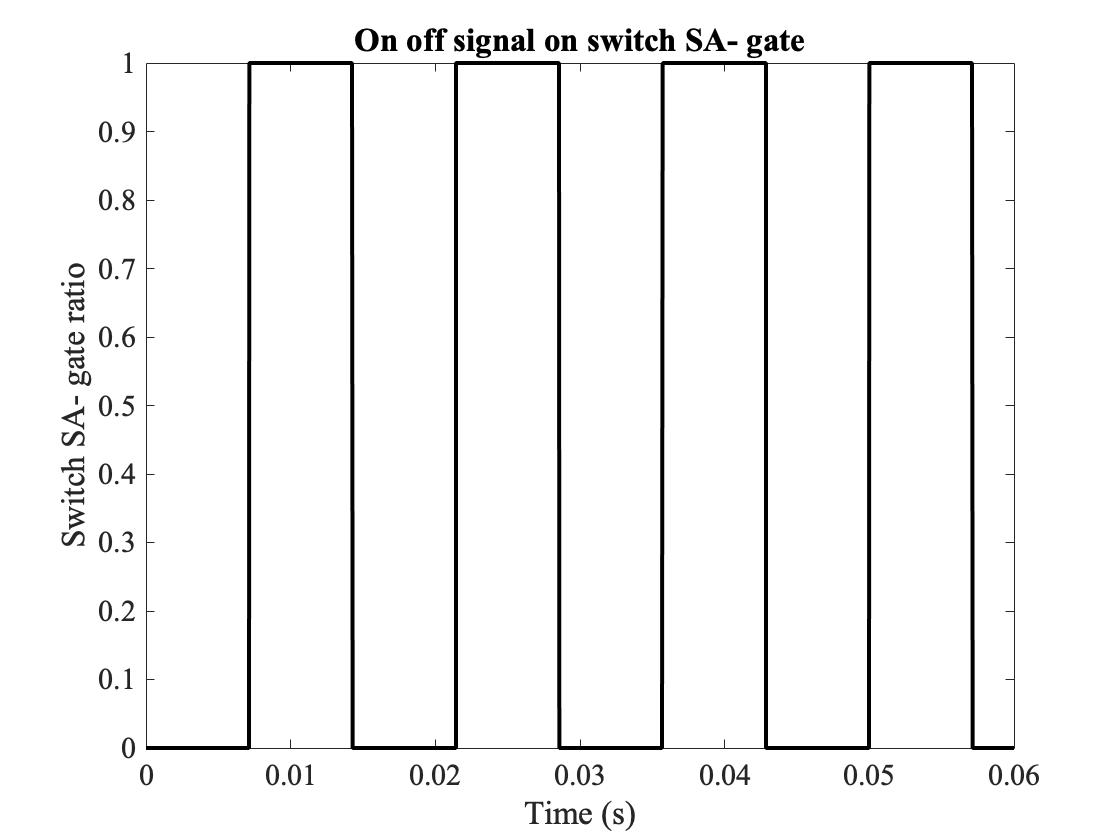
\includegraphics[scale=0.15]{SwitchDAN.jpg}
\caption{SW- gate signal}
\label{fig:s2}
\end{subfigure}%
\begin{subfigure}{.5\textwidth}
  \centering
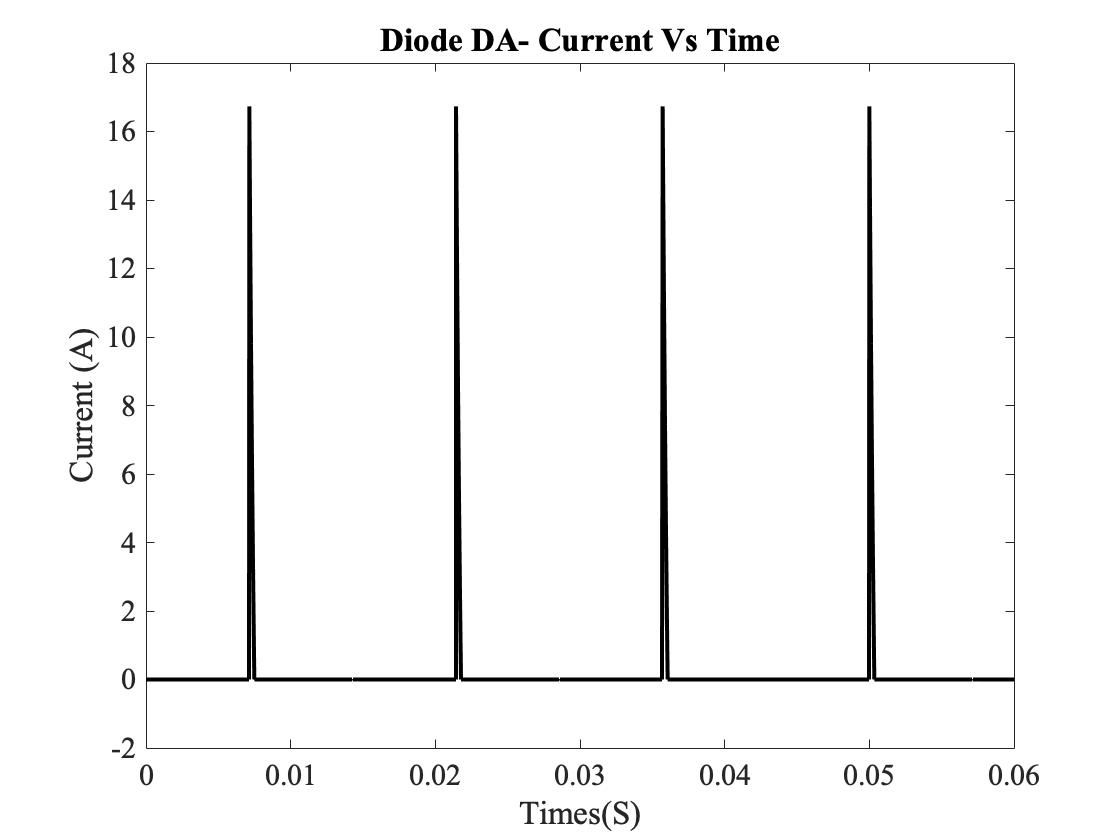
\includegraphics[scale=0.15]{1c.jpg}
\caption{Diode DA- Current}
\label{fig:s3}
\end{subfigure}
\caption{SW-switch frequency and DA- current simulation results}
\label{fig:fig3}
\end{figure}

Figure:\ref{fig:s2} shows the gate drive signal on the SA- IGBT oscillating at the frequency of the driving and desired output sine wave at $70Hz$. The diode DA- conduction is shown in Figure:\ref{fig:s3}, here the inductor $L_a$ forces current to flow through DA- when the switch SA+ turns off, the energy stored in the inductor is dissipated through the resistor and forced in the opposite direction from the voltages applied through the other phases until the inductor is counteracted and current flows in the opposite direction. 

From the graph we can measure the diode conduction time at $345\mu s$.

\section*{2a} 
Choose SPWM as we can vary the output voltage by changing the amplitude of the input voltage sinusiod. SPWM maximum fundamental is given by $V_{Ph}=\frac{1}{2}$ meaning a maximum fundamental component using SPWM of 250V can be achieved. This means we must overmodulate into saturation, being in saturation constantly would be six step mode, the fundamental component using six step is given by $V_{Ph}=\frac{2 }{\pi}$ giving 318V meaning a SPWM model going into saturation would meet our specification of variable and between 200 and 280V.

\section*{2b} 
When undermodulating with a sine wave voltage of 0.8V we get the 200V output seen in Figure:\ref{fig:2b1a}. The FFT shown in Figure:\ref{fig:2b1b} has the output fundamental peak at 200V with bands later peaking around the sampling frequency.

200V 0.8V in

280V 1.25V in


\begin{figure}[H]
\begin{subfigure}{.5\textwidth}
  \centering
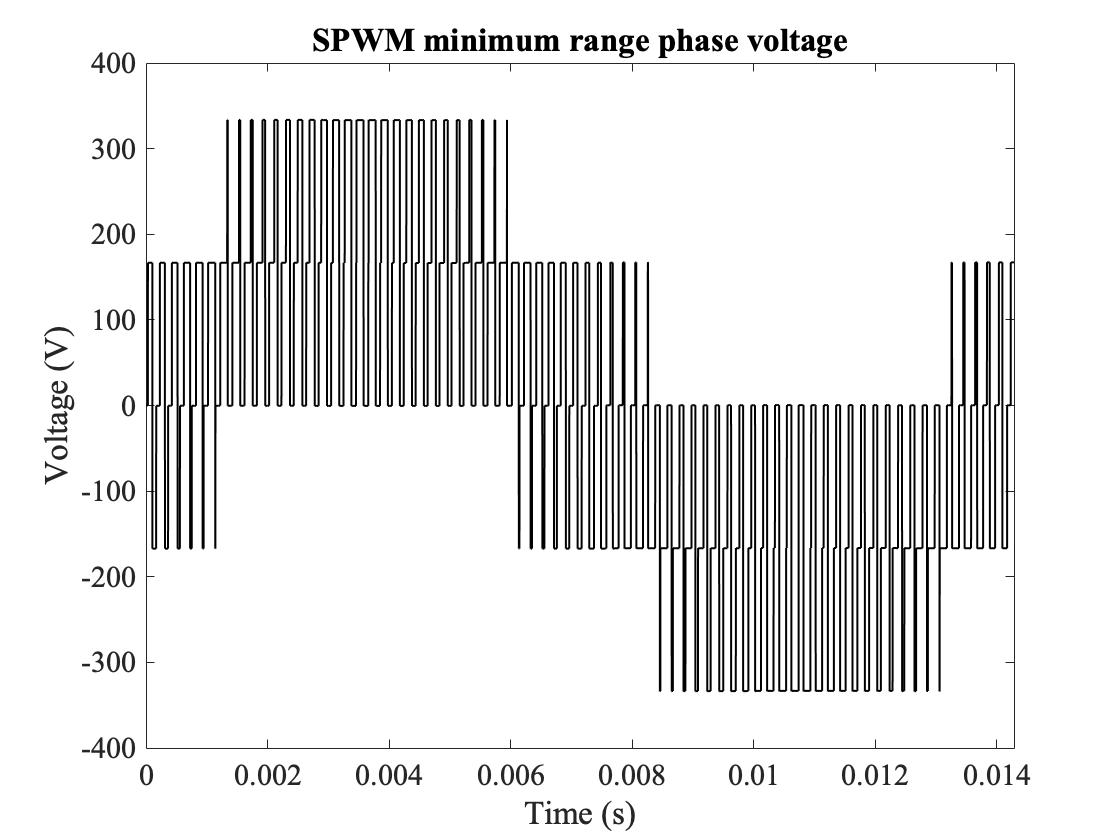
\includegraphics[scale=0.15]{2b1.jpg}
\caption{minimum SPWM voltage signal}
\label{fig:2b1a}
\end{subfigure}%
\begin{subfigure}{.5\textwidth}
  \centering
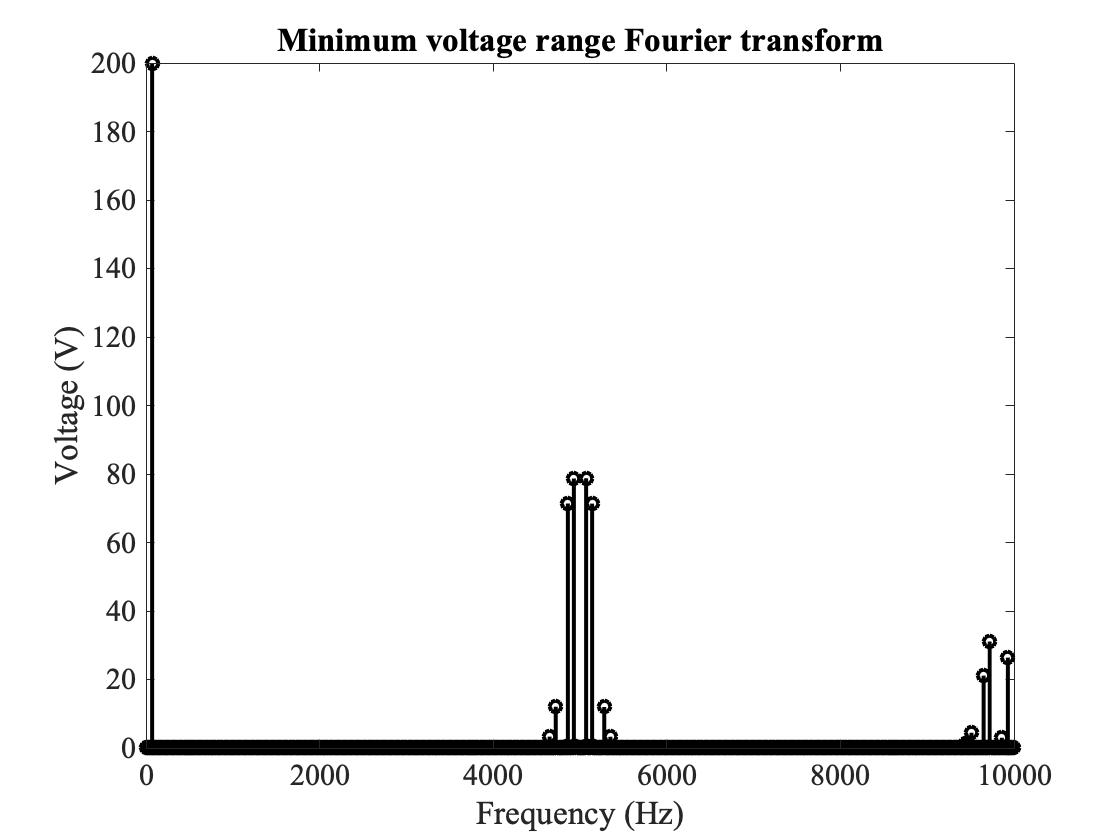
\includegraphics[scale=0.15]{2b2.jpg}
\caption{FFT of signal in Figure:\ref{fig:2b1a}}
\label{fig:2b1b}
\end{subfigure}
\caption{}
\label{fig:fig4}
\end{figure}
When overmodulating the input sinewave to 1.25V we get the results shown in Figure:\ref{fig:fig5} where the fundamental magnitude is 280V, when overmodulating the surrounding frequencies magnitudes increase meaning that if low pass filtered there will be noticeable distortion to the signal.
\begin{figure}[H]
\begin{subfigure}{.5\textwidth}
  \centering
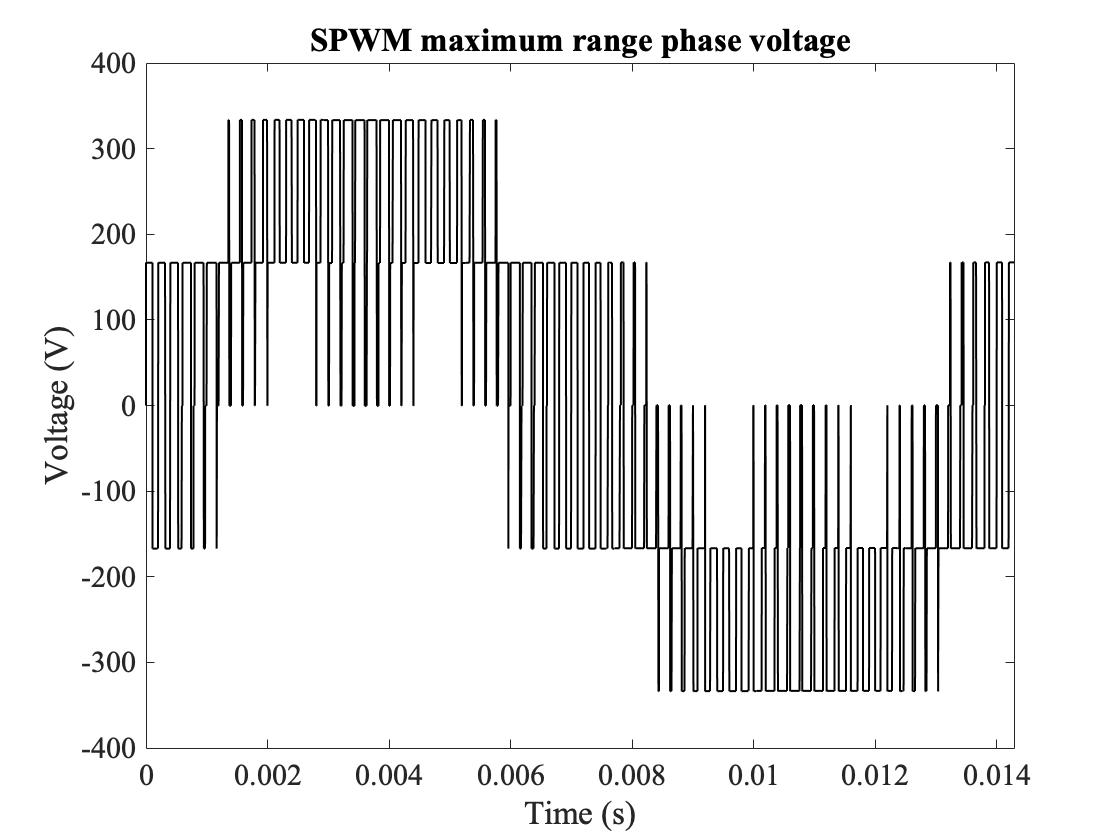
\includegraphics[scale=0.15]{2b3.jpg}
\caption{maximum SPWM voltage signal}
\label{fig:22ba}
\end{subfigure}%
\begin{subfigure}{.5\textwidth}
  \centering
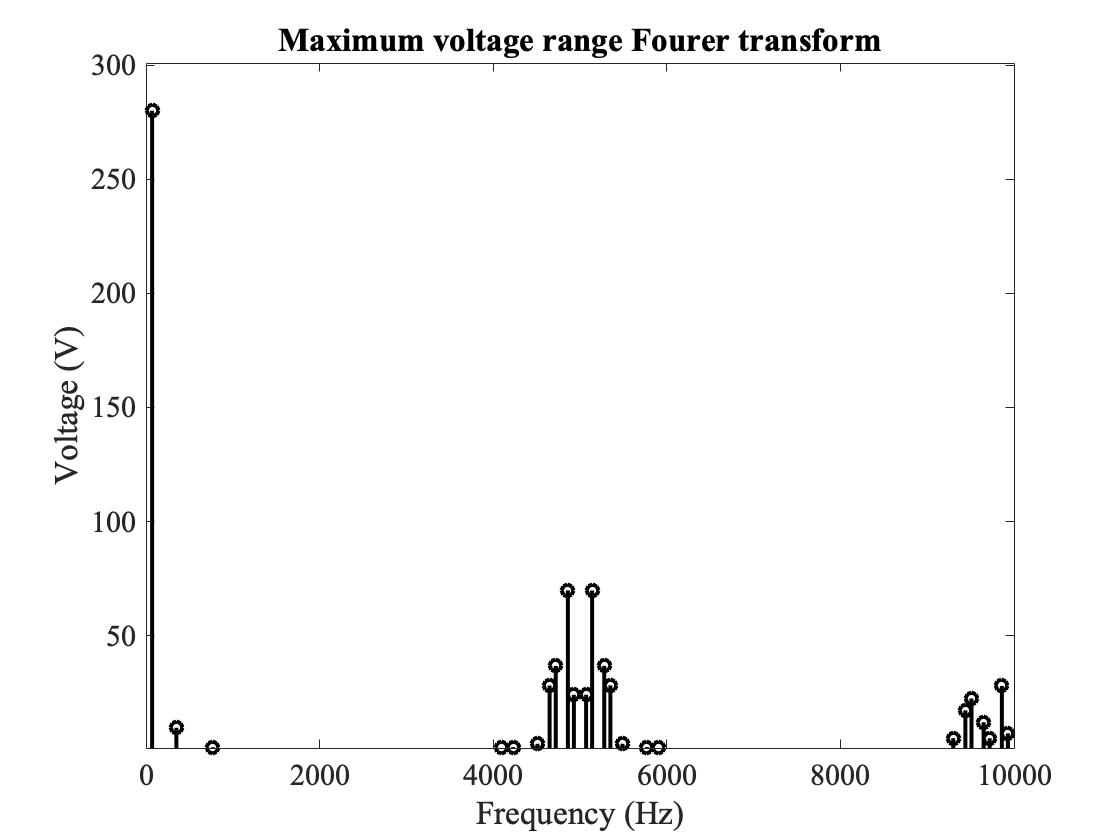
\includegraphics[scale=0.15]{2b4.jpg}
\caption{FFT of signal in Figure:\ref{fig:22ba}}
\label{fig:fftOne}
\end{subfigure}
\caption{}
\label{fig:fig5}
\end{figure}

\section*{2c}

The dead time signal is shown in Figure:\ref{fig:2ca} with the corresponding FFT in Figure:\ref{fig:2cb}. We can see the output is set at 180V but now extra artifacts can be seen at a noticeable magnitude close to the fundamental frequency meaning the signal will be noticeably distorted.

\begin{figure}[H]
\begin{subfigure}{.5\textwidth}
  \centering
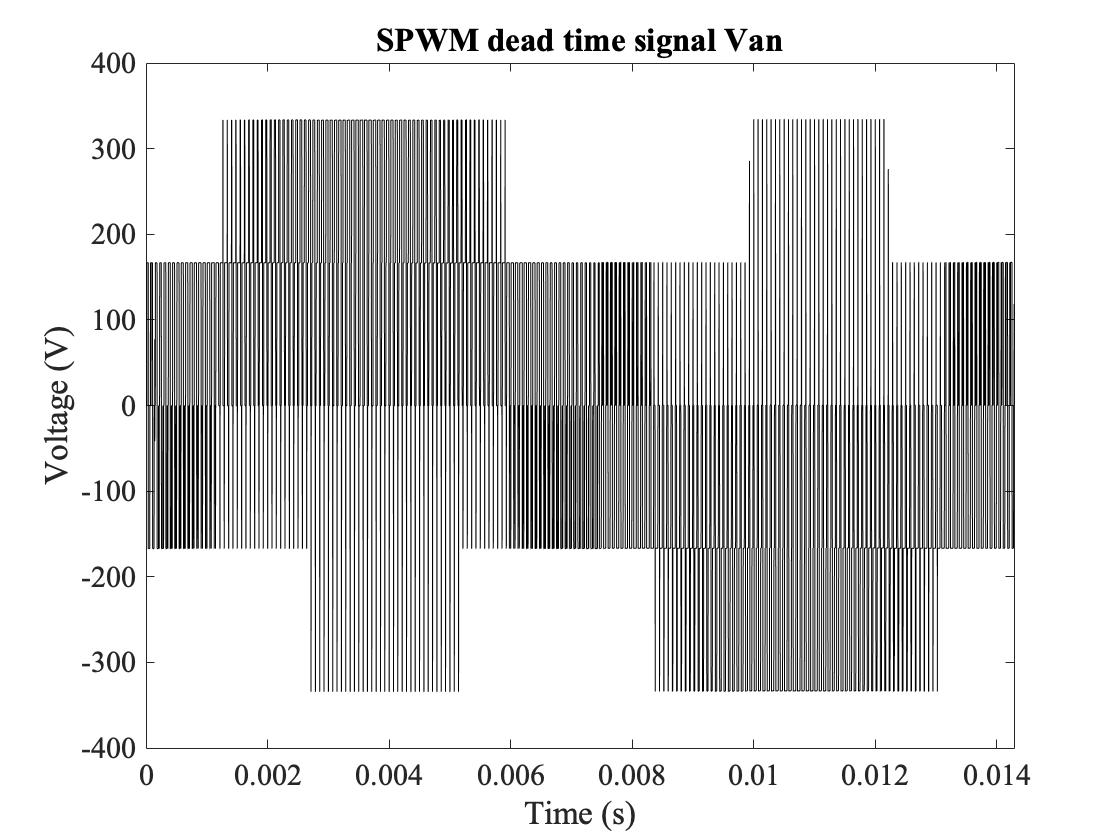
\includegraphics[scale=0.15]{2c1.jpg}
\caption{Output voltage $V_{an}$ with $3\mu s$ dead time}
\label{fig:2ca}
\end{subfigure}%
\begin{subfigure}{.5\textwidth}
  \centering
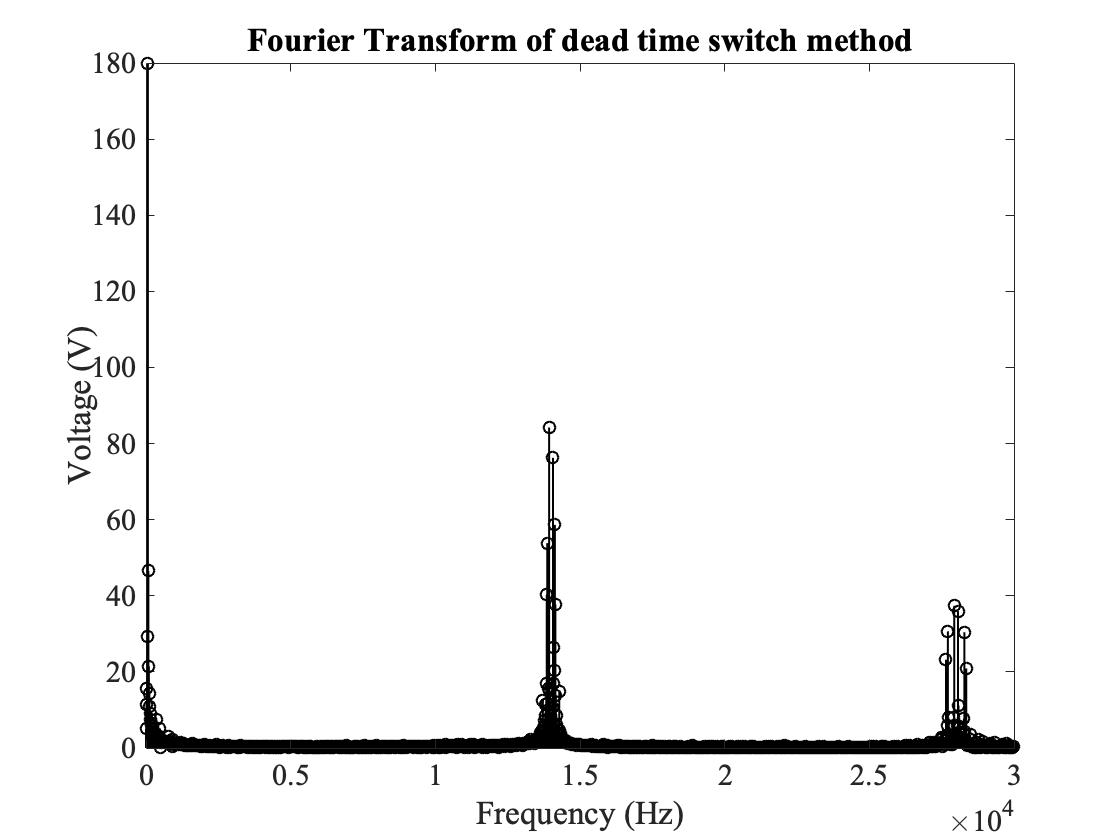
\includegraphics[scale=0.15]{2c2.jpg}
\caption{FFT of signal in Figure:\ref{fig:2ca}}
\label{fig:2cb}
\end{subfigure}
\caption{}
\label{fig:fig6}
\end{figure}

The larger a circuits power factor is the larger the inductance is compared to the circuit resistance, as this increases the circuits ability to drive a constant output current increases smoothing the output current through dead time forcing the output closer to a sine wave.

In Figure:\ref{fig:deadTimePF} we can see the effect of power factor on fundamental frequency magnitude is an almost linear relationship rising the magnitude the larger the inductance compared to the resistance as expected.  


\begin{figure}
    \centering
    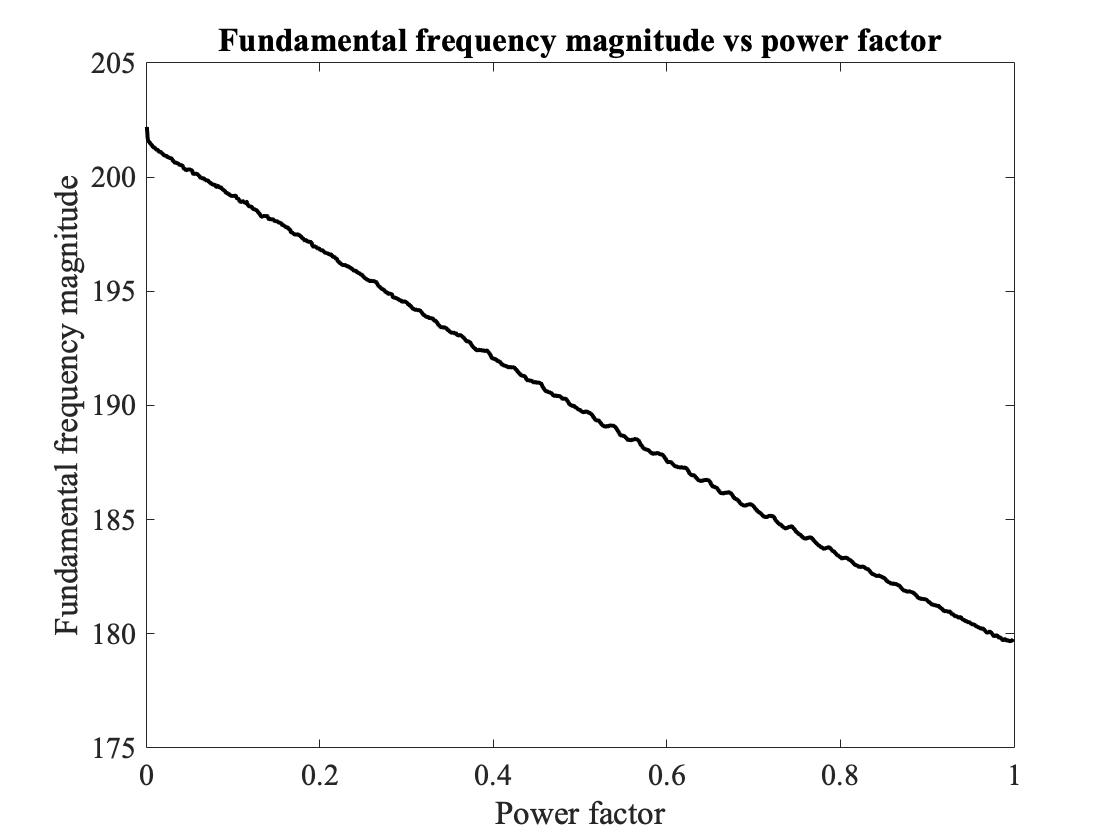
\includegraphics[scale=0.2]{2c3.jpg}
    \caption{$3\mu s$ dead time first fundamental magnitude vs power factor}
    \label{fig:deadTimePF}
\end{figure}



\bibliographystyle{plain}
\end{document}

